\section{Concept Map}

Das Thema der vorliegenden Arbeit ist die Ausarbeitung des Algorithmus der Breitensuche in Form Leitprogrammartiger Unterrichtsunterlagen (LPU) für das Gymnasium.  
Zu diesem Zweck wurde folgende Concept-Map (s. Abb.~\ref{fig:cmap}) entworfen, die sowohl das Vorwissen als auch einen kleinen Ausblick auf weitere Themen geben soll.
Dabei wurden Konzepte blau gefärbt, welche als Vorwissen schon bekannt sein sollten, aber im Rahmen dieser Arbeit nochmal wiederholt werden. 
Neue Konzepte wurden grün eingefärbt und werden in dieser Arbeit behandelt bzw. eingeführt.
Weitere Konzepte, die nicht mehr in dieser Arbeit behandelt werden, wurden orange gefärbt. 
Insbesondere m"ochten wir die Darstellung von Graphen in Form von Adjazenmatrizen wiederholen und fundiert mit den SuS besprechen. 
Deshalb wurde das Konzept \emph{gr"un} gef"arbt. 
Wir haben uns bewusst f"ur die Darstellung mit Adjazenzmatrizen entschieden, da wir dieses f"ur den Algorithmus der Breitensuche ben"otigen. 
Alternativ kann man auch Adjazenzlisten (\emph{orange}) verwenden.
Beide Konzepte sind aber Listen von Listen und f"ur SuS nicht trivial.

\begin{figure}[htb]
\begin{center}
%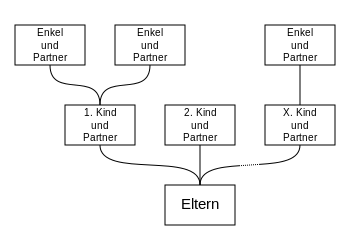
\includegraphics[width=.7\textwidth]{../fig/stammbaum.png}
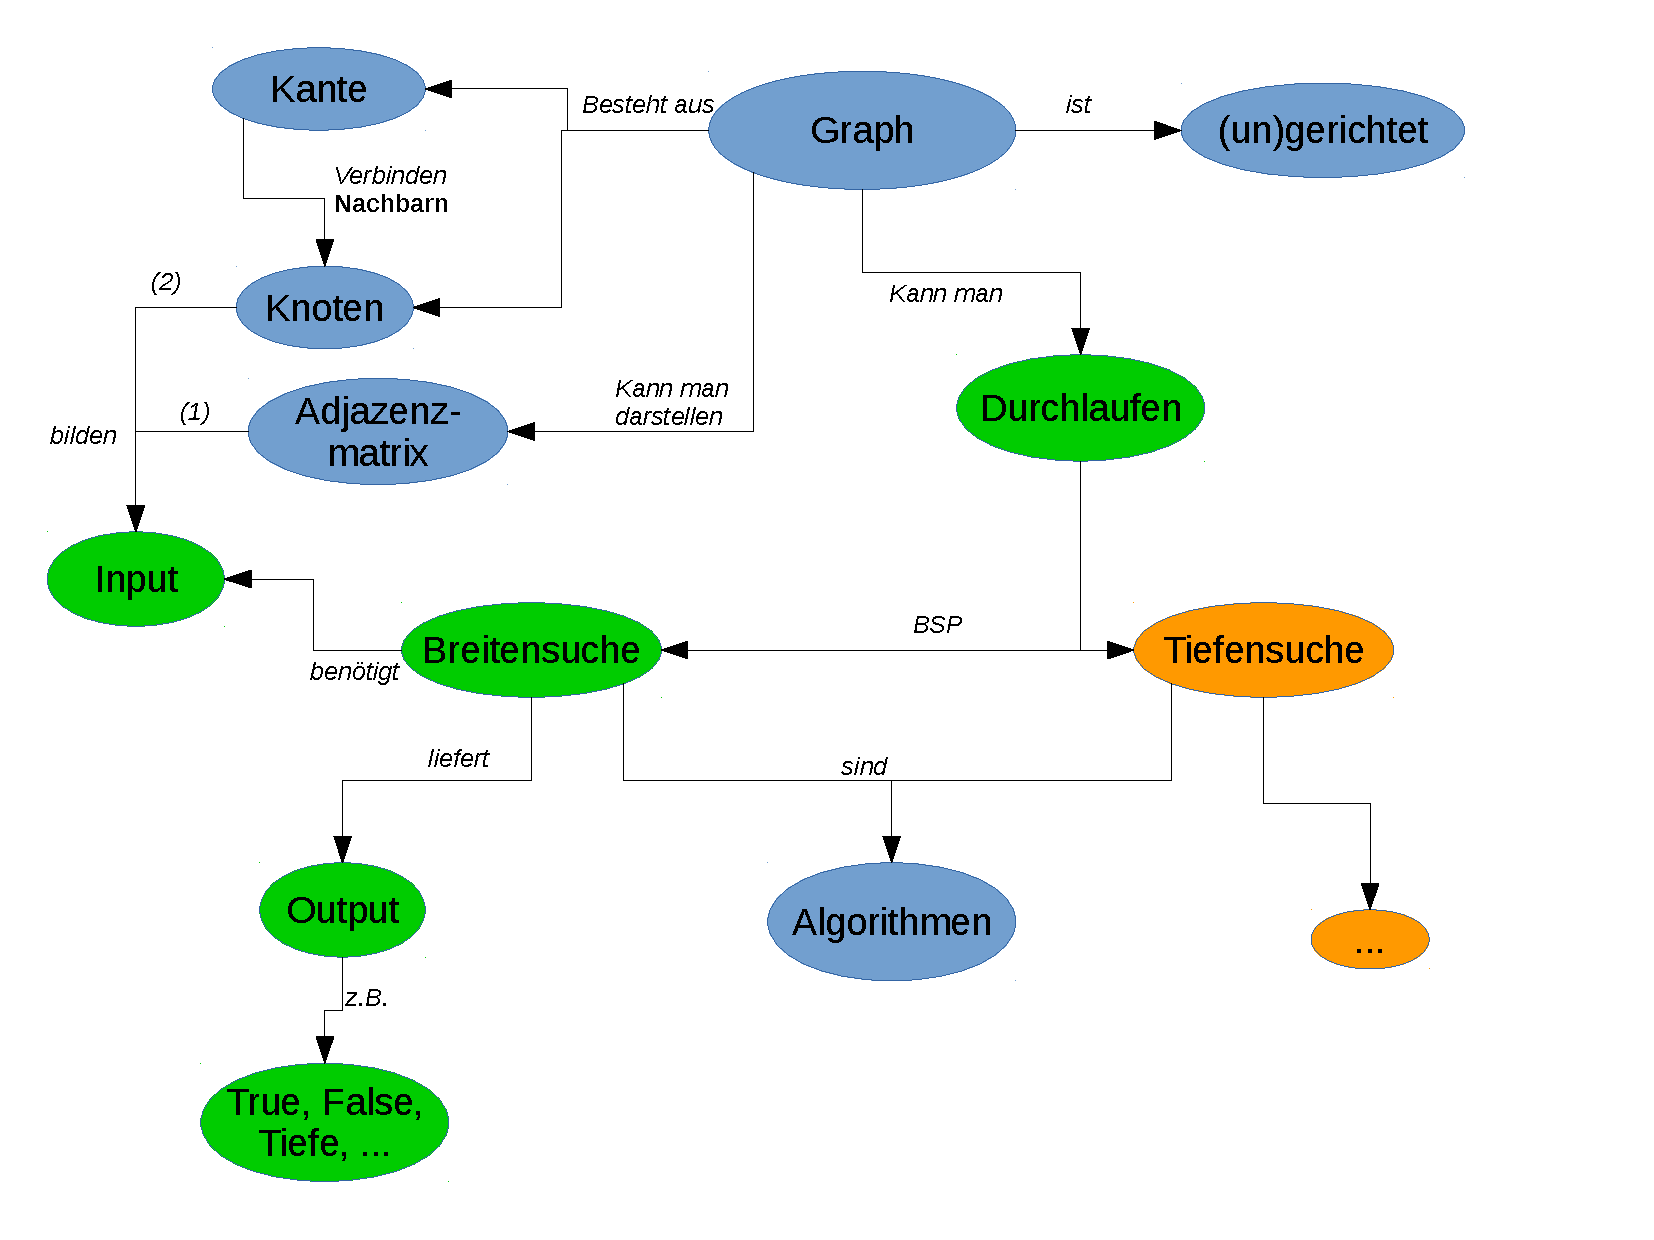
\includegraphics[width=.99\textwidth]{../cmap/bsuche_cmap.pdf}
\caption{Concept-Map zum Thema Breitensuche.
Blaue Konzepte und grüne Konzept werden in dieser Arbeit behandelt, wobei die Blauen das Vorwissen abbilden und Grüne neue Konzepte sind. 
Orangene Konzepte bilden einen Ausblick auf Konzepte, welche im Rahmen dieser Arbeit nicht mehr behandelt werden. 
}
\label{fig:cmap}
\end{center}
\end{figure}

Aus dieser Concept Map ergibt sich eine Sequenzierung des Unterrichts, bei dem zuerst die grundlegenden Begriffe eines Graphen repetiert werden, damit das Vorwissen der Sch\"uler aktiviert wird. Darauf aufbauend werden dann die neuen Konzepte eingef\"uhrt. Ein kurzer inhaltlicher \"Uberblick dieser Sequenzierung wird in Kapitel \ref{lpu:inhalt} vorgestellt.

\section{Aufbau der LPU}

\subsection{F\"ur wen sind die LPU geeignet?}
Die Unterlagen richten sich an Sch\"ulerinnen und Sch\"uler der Gymnasialstufe (11. oder 12. Schuljahr) und sind f\"ur den Informatikunterricht im Erg\"anzungsfach Informatik geeignet, idealerweise f\"ur Sch\"uler mit mathematisch/naturwissenschaftlichem Schwerpunkt. 
Die vorliegenden Unterlagen sollten im zweiten Quartal des Erg\"anzungsfaches Informatik eingesetzt werden k\"onnen.


\subsection{Vorwissen}

Es wird davon ausgegangen, dass die Sch\"uler bereits einige Grundlagen der Informatik kennengelernt haben, insbesondere den Begriff Algorithmus. Zum Vorwissen der Sch\"uler sollte ausserdem der Begriff des Graphen geh\"oren. Dieses Vorwissen soll zu Beginn nochmals aktiviert werden. Dabei werden die wichtigsten Begriffe repetiert: der Aufbau eines Graphen aus Knoten und Kanten, gerichtete und ungerichtete Graphen sowie der Begriff von Nachbarsknoten. Damit wird eine klare Basis f\"ur die in den Unterlagen verwendeten Begriffe geschaffen.

Der Begriff des Algorithmus wird als Vorwissen vorausgesetzt, aber nicht nochmals aktiviert bzw. repetiert, da davon ausgegangen wird, dass sich die Sch\"uler schon vertiefter mit dem Begriff auseinandergesetzt haben und im Rahmen des Erg\"anzungsfaches Informatik schon verschiedene Algorithmen kennengelernt bzw. entwickelt haben. 
Die SuS k"onnen Algorithmen in Form von Pseudocode lesen und selber verfassen.


F\"ur die Implementationen und die Programmier\"ubungen werden keine Details repetiert, da die Sch\"uler auch hier im Rahmen des Erg\"anzungsfaches bereits einige Programme implementiert und die Grundlagen von Datentypen, Kontrollstrukturen und modularem Aufbau kennengelernt und viel ge\"ubt haben sollten. 
Wichtig sind f\"ur die Programmieraufgaben in diesen Unterlagen unter anderem Unterprogramme, Arrays und Schleifen.
Zus\"atzlich sollen die Sch\"uler  wissen, wie Programme modular aufgebaut werden k"onnen und bereits in der Lage sein, einfache Programme in TigerJython zu schreiben. 

Die Darstellung der Graphen als Listen von Listen in Python wird explizit repetiert.


Neue Begriffe und Konzepte werden in den Unterlagen so eingef\"uhrt, dass sie am vorhandenen Wissen ankn\"upfen und dieses erweitern.

\subsection{Konzeption}
Die Unterlagen sind so aufgebaut, dass schrittweise neue Konzepte eingef\"uhrt und erläu-tert werden. Im Fokus soll die Entwicklung beziehungsweise F\"orderung des Algorithmischen Denkens stehen. Die Sch\"uler sollen nicht nur das Konzept und die Anwendung der Breitensuche kennenlernen, sondern auch lernen, wie ein Algorithmus entwickelt wird und wie ein Algorithmus formuliert werden soll, damit er f\"ur eine breite Klasse von Problemen eingesetzt werden kann. Die LPU sollen dazu beitragen, dass die Sch\"uler sich intensiv mit der Formulierung der Problemstellung sowie der Entwicklung des Algorithmus auseinandersetzen und schlussendlich auch in der Lage sind, den Algorithmus zu implementieren.


\section{Lernziele}

Aus der Concept-Map lassen sich folgende Lernziele für diese Arbeit ableiten. 

\subsection{Leitidee}

Graphen spielen eine wichtige Rolle in unserem Alltag und werden sehr häufig zur Darstellung von Zusammenhängen verwendet (S-Bahnnetzwerk, Facebook, Websites, \dots). 
Mit diesen Netzwerken sind viele Fragen verbunden: Über wie viel Freundschaften bin ich mit einer anderen Person verbunden? Wie lange ist die kürzeste Verbindung von A nach B?
Damit man ein grundlegendes Verständnis dafür entwickelt, muss man sich überlegen, wie man Graphen durchsuchen kann. 
Dies kann man erreichen indem man in der Breite oder in der Tiefe sucht. 
Mithilfe der Breitensuche soll ein elementarer Einstieg aufgezeigt werden, an dem man auch das algorithmische Denken fördern kann.

Graphen sind aber nicht nur \glqq sch"one\grqq\ Objekte, sonder mithilfe dieser k"onnen wir Probleme mathematisch modellieren. 
Viele Probleme lassen sich auf Graphen reduzieren (SAT~\cite{hrom1}) und sind ein grundlegendes Werkzeug um Probleme zu klassifizieren. 


\subsection{Dispositionsziel}

Die SuS wissen, dass man gewisse Probleme mit Hilfe von Graphen modellieren und mit Graphenalgorithmen lösen kann. 
Sie können analysieren und beurteilen, ob Problemstellungen mithilfe einer Breitensuche in einem Graphen gelöst werden können.



\subsection{Operationalisierte Lernziele}

Die folgenden Lernziele richten sich nach den Ebenen der revidierten Lernzieltaxonomie~\cite{krathwohl}: Wissen (K1), Verstehen (K2), Anwenden (K3), Analysieren (K4), Evaluieren (K5), Erschaffen (K6).

Nach dieser Einheit können die SuS \dots

\begin{enumerate}
\item \dots die Begriffe und Unterschiede zur Darstellung von einfachen Graphen verstehen: (un)gerichtet, Knoten und Kante. (K2)

\item \dots verschiedene Darstellungsmöglichkeiten von Graphen aufzählen und diese ineinander überführen: Zeichnung, Knoten-/ Kantenmenge und Adjazenzmatrix. (K1)

\item \dots die Nachbarn von Knoten auf verschieden Darstellungen von Graphen bestimmen. (K3)

\item \dots ein Programm schreiben, welches die Nachbarknoten eines bestimmten Knotens in einer Adjazenzmatrix ausgibt. (K3)

\item\dots ein gegebenes Problem analysieren und mit einem Graphen modellieren. (K4)
 
\item \dots die Funktionsweise einer Breitensuche in einem Graphen beschreiben. (K1)

\item\dots f\"ur einen Graphen mittels Breitensuche beurteilen, ob ein Knoten von einem anderen Knoten aus erreichbar ist. (K3)

\item\dots f\"ur einen Graphen mittels Breitensuche den k\"urzesten Weg von einem Knoten zu einem anderen Knoten finden (in Bezug auf die Anzahl Kanten, die traversiert werden m\"ussen). (K3)

\item\dots f\"ur einen Graphen mittels Breitensuche eine Folge von Knoten angeben, welche auf k\"urzestem Weg von einem Knoten zu einem anderen Knoten f\"uhren. (K3)

\item \dots ein gegebenes Problem mit einem Graphen modellieren und mittels Breitensuche eine passende Lösung des Problems finden. (K6)

\item \dots den in Pseudocode formulierten Algorithmus der Breitensuche in einem Programm in TygerJython implementieren. (K3)


\end{enumerate}

\section{Sequenzierung der Unterrichtseinheit}\label{lpu:inhalt}

Aus der Concept-Map und den Lernzielen ergibt sich folgender Ablauf für die LPU:
Zuerst m"ochten wir die SuS f"ur das Thema motivieren und abholen.
Der \emph{kognitiv aktivierene Einstieg} in ein neues Thema wird u.a. in~\cite{stern1} empfohlen.
Dazu pr"asentieren wir das Problem des k"urzesten Weges im "OV. 
Anhand dessen zeigen wir dann auf, dass wir zuerst gewisse Konzepte wiederholen und erweitern m"ussen, um dieses Problem zu l"osen.

In einem ersten Abschnitt werden also nochmal die Grundlagen zu Graphen und ihrer Darstellungen wiederholt und anhand von Beispielen und Aufgaben geübt. 
Dabei wird darauf geachtet zuerst eine zeichnerische Darstellung, dann eine Mengendarstellung und zum Schluss die Adjazenzmatrix einzuführen. 
Hierbei wurde sich an \cite{cormen,ottmann} orientiert.
Zum Schluss des ersten Abschnitts soll mit der Einführung von Nachbarn und dem Schreiben eines solchen Programms eine Vorarbeit für den kommenden Abschnitt gelegt werden.

Im zweiten Abschnitt werden Grundlagen \"uber das Modellieren von Problemen mit Hilfe von Graphen und das L\"osen der Probleme mit Hilfe von Graphenalgorithmen vermittelt. Insbesondere werden Problemstellungen betrachtet, die sich mit Hilfe von der Breitensuche l\"osen lassen. Der Algorithmus f\"ur die Breitensuche wird Schritt f\"ur Schritt erarbeitet, erweitert und implementiert sowie an konkreten Beispielen angewendet. F\"ur den Algorithmus wird ein Vorgehen mit F\"arben von Knoten verwendet, wie es auch in \cite{cormen} zu finden ist.